\documentclass[conference]{IEEEtran}
\IEEEoverridecommandlockouts

\usepackage{graphicx}
\usepackage{booktabs}
\usepackage{amsmath}
\usepackage{url}

\begin{document}

\title{An Offline Voice-Based Nepali Student Assistant Using Machine Learning for Low-Resource Immediate Systems}

\author{\IEEEauthorblockN{Risesh Shtha}
\IEEEauthorblockA{Department of Computing\\
Softwarica College of IT \& E-Commerce (In Collaboration with Coventry University)\\
Kathmandu, Nepal\\
student@softwarica.edu.np}
}

\maketitle

\begin{abstract}
This paper presents the design, implementation, and evaluation of an offline, voice-enabled educational assistant for Nepali-speaking students. The system targets low-resource learning environments in Nepal by integrating offline automatic speech recognition (ASR), Support Vector Machine (SVM)-based intent classification, and knowledge-base retrieval into a single prototype. A custom dataset of 2{,}150 Nepali question-answer pairs sourced from primary school textbooks across six subject intents (Science, Social Studies, Nepali Language, Health, Physical Education, and Arts) was cleaned and used for training and evaluation. The intent classifier uses TF-IDF character n-gram features and an optimized Linear SVM pipeline (TF-IDF char n-grams + TruncatedSVD + SMOTE + GridSearchCV). On a held-out test set ($n=430$), the final model achieved 74.65\% accuracy with macro F1 of 77.53\%. Inference benchmarking measured a mean end-to-end (intent + retrieval) latency of 21.9\,ms per query on CPU, supporting real-time offline use. The full system includes a Tkinter GUI, microphone input with Faster-Whisper ASR, and Nepali text-to-speech via eSpeak-NG.
\end{abstract}

\begin{IEEEkeywords}
Nepali NLP, offline voice assistant, intent classification, TF-IDF, linear SVM, SMOTE, Faster-Whisper, edge deployment.
\end{IEEEkeywords}

\section{Introduction}
Nepal faces a persistent gap in accessible Nepali-language educational technology, especially in rural contexts where internet access and learning resources are limited. Most mainstream voice assistants rely on cloud services and are optimized for high-resource languages, which reduces their usefulness for Nepali students requiring immediate, offline support. This project investigates whether a lightweight machine learning pipeline can deliver practical intent classification for Nepali educational questions and connect that intent to an offline knowledge base for answer retrieval.

This work contributes: (i) an end-to-end offline prototype for Nepali student assistance (ASR $\rightarrow$ intent classification $\rightarrow$ retrieval $\rightarrow$ TTS), (ii) a cleaned Nepali educational Q\&A dataset (2{,}150 samples; six subject intents), (iii) an optimized Linear SVM intent classifier using TF-IDF character n-gram features, and (iv) evaluation evidence including accuracy/F1, confusion matrix, and latency benchmarking artifacts.

\section{The Data Set}
\subsection{Problem Definition}
The primary machine learning task is multi-class intent classification. Given a Nepali query $q$, the classifier predicts one intent label $y$ from:
\[
\{\texttt{arts\_question},\texttt{health\_question},\texttt{nepali\_language\_question},\texttt{physical\_education\_question},\texttt{science\_question},\texttt{social\_question}\}.
\]
The predicted label is then used to narrow the search space for offline answer retrieval from a local knowledge base of textbook Q\&A pairs.

\subsection{Dataset Source and Composition}
Because no suitable public Nepali educational Q\&A dataset aligned to the intended subject-specific intents was available for this prototype, a custom dataset was constructed from Nepali primary school textbooks (Grades 4--7), producing 2{,}150 cleaned question--answer samples with intent labels.

\subsection{Class Distribution}
The dataset contains moderate class imbalance (Science and Social Studies dominate). Table~\ref{tab:intentdist} summarizes sample counts.

\begin{table}[ht]
\caption{Dataset Summary (Intent Distribution)}
\label{tab:intentdist}
\centering
\begin{tabular}{lrr}
\toprule
Intent Class & Samples & \% of Total \\
\midrule
\texttt{science\_question} & 686 & 31.9 \\
\texttt{social\_question} & 622 & 28.9 \\
\texttt{nepali\_language\_question} & 549 & 25.5 \\
\texttt{health\_question} & 152 & 7.1 \\
\texttt{physical\_education\_question} & 77 & 3.6 \\
\texttt{arts\_question} & 64 & 3.0 \\
\midrule
\textbf{Total} & \textbf{2{,}150} & \textbf{100.0} \\
\bottomrule
\end{tabular}
\end{table}

\section{Data Preparation}
\subsection{Text Normalization}
The dataset is cleaned using a Devanagari-aware normalization routine (implemented in \texttt{codes/data\_prep.py}), including removal of leading Nepali/ASCII numbering patterns, removal of repeated instructional noise phrases (e.g., common ``write/tell'' instruction words), dropping null/short questions, and standardizing column names.

\subsection{Train/Test Split}
An 80/20 stratified split is used with fixed random seed (\texttt{random\_state=42}), resulting in 1{,}720 training and 430 test samples.

\subsection{Feature Representation}
The intent classifier uses TF-IDF character word-boundary n-grams (analyzer=\texttt{char\_wb}, ngram\_range=(2,4), sublinear\_tf=True). Character n-grams are selected to be robust to Nepali morphology, spelling variation, and ASR noise.

\subsection{Class Imbalance Handling}
Two complementary strategies address imbalance: \texttt{class\_weight='balanced'} in LinearSVC and SMOTE oversampling within the training pipeline (applied inside cross-validation folds to avoid leakage).

\begin{figure}[ht]
\centering
\includegraphics[width=\linewidth]{../outputs/eda_intent_dist.png}
\caption{Intent class distribution after cleaning (2{,}150 samples).}
\label{fig:eda}
\end{figure}

\section{Machine Learning Classification Technique}
This project focuses on a single model family for intent classification: a Linear Support Vector Machine (\texttt{LinearSVC}) trained on TF-IDF character n-gram features. The optimized pipeline uses TruncatedSVD (dimensionality reduction; enables dense-space SMOTE), SMOTE oversampling, and 5-fold stratified GridSearchCV to tune $C$ and n-gram range.

\section{Application and Results}
\subsection{Implementation and Prototype}
The prototype is implemented in Python and includes: offline ASR using Faster-Whisper with CPU INT8 inference, intent classification using the trained optimized Linear SVM, offline answer retrieval via TF-IDF cosine similarity restricted by predicted intent, offline TTS using eSpeak-NG (fallback to \texttt{pyttsx3}), and a Tkinter GUI (\texttt{codes/app.py}) supporting typed and microphone input.

\subsection{Overall Results (Optimized SVM)}
Evaluation metrics are reported on the held-out test set ($n=430$) and recorded in \texttt{outputs/eval\_report.json}:
\begin{itemize}
  \item Accuracy: 74.65\%
  \item Macro F1: 77.53\%
  \item Weighted F1: 74.64\%
\end{itemize}

\begin{figure}[ht]
\centering
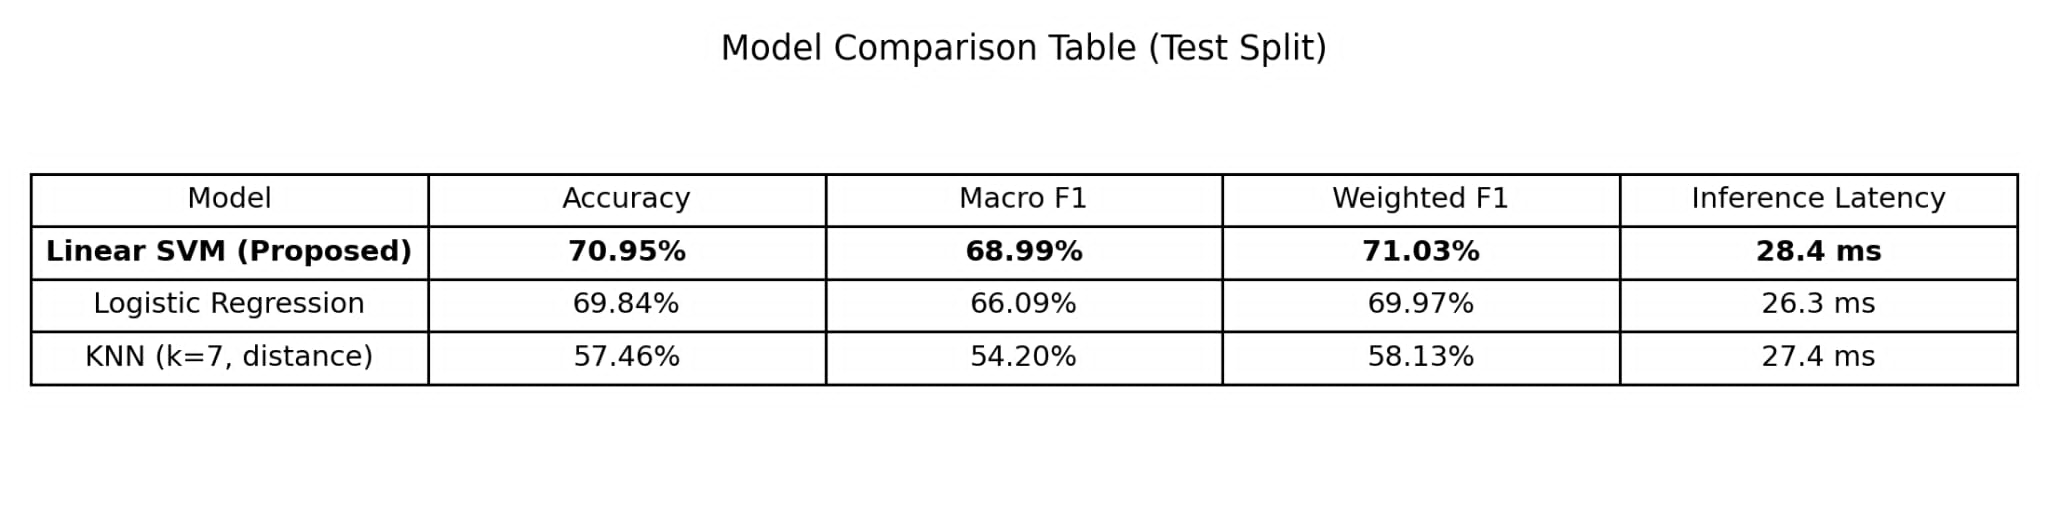
\includegraphics[width=\linewidth]{../outputs/accuracy_table.png}
\caption{Overall test metrics for the final SVM model.}
\label{fig:acctable}
\end{figure}

\subsection{Per-Class Results}
Table~\ref{tab:perclass} shows per-class precision, recall, F1, and support for the optimized SVM.

\begin{table}[ht]
\caption{Per-Class Performance (Optimized SVM)}
\label{tab:perclass}
\centering
\begin{tabular}{lrrrr}
\toprule
Intent & Precision & Recall & F1 & Support \\
\midrule
\texttt{arts\_question} & 0.923 & 0.923 & 0.923 & 13 \\
\texttt{health\_question} & 0.760 & 0.633 & 0.691 & 30 \\
\texttt{nepali\_language\_question} & 0.755 & 0.700 & 0.726 & 110 \\
\texttt{physical\_education\_question} & 0.917 & 0.733 & 0.815 & 15 \\
\texttt{science\_question} & 0.767 & 0.745 & 0.756 & 137 \\
\texttt{social\_question} & 0.690 & 0.800 & 0.741 & 125 \\
\bottomrule
\end{tabular}
\end{table}

\begin{figure}[ht]
\centering
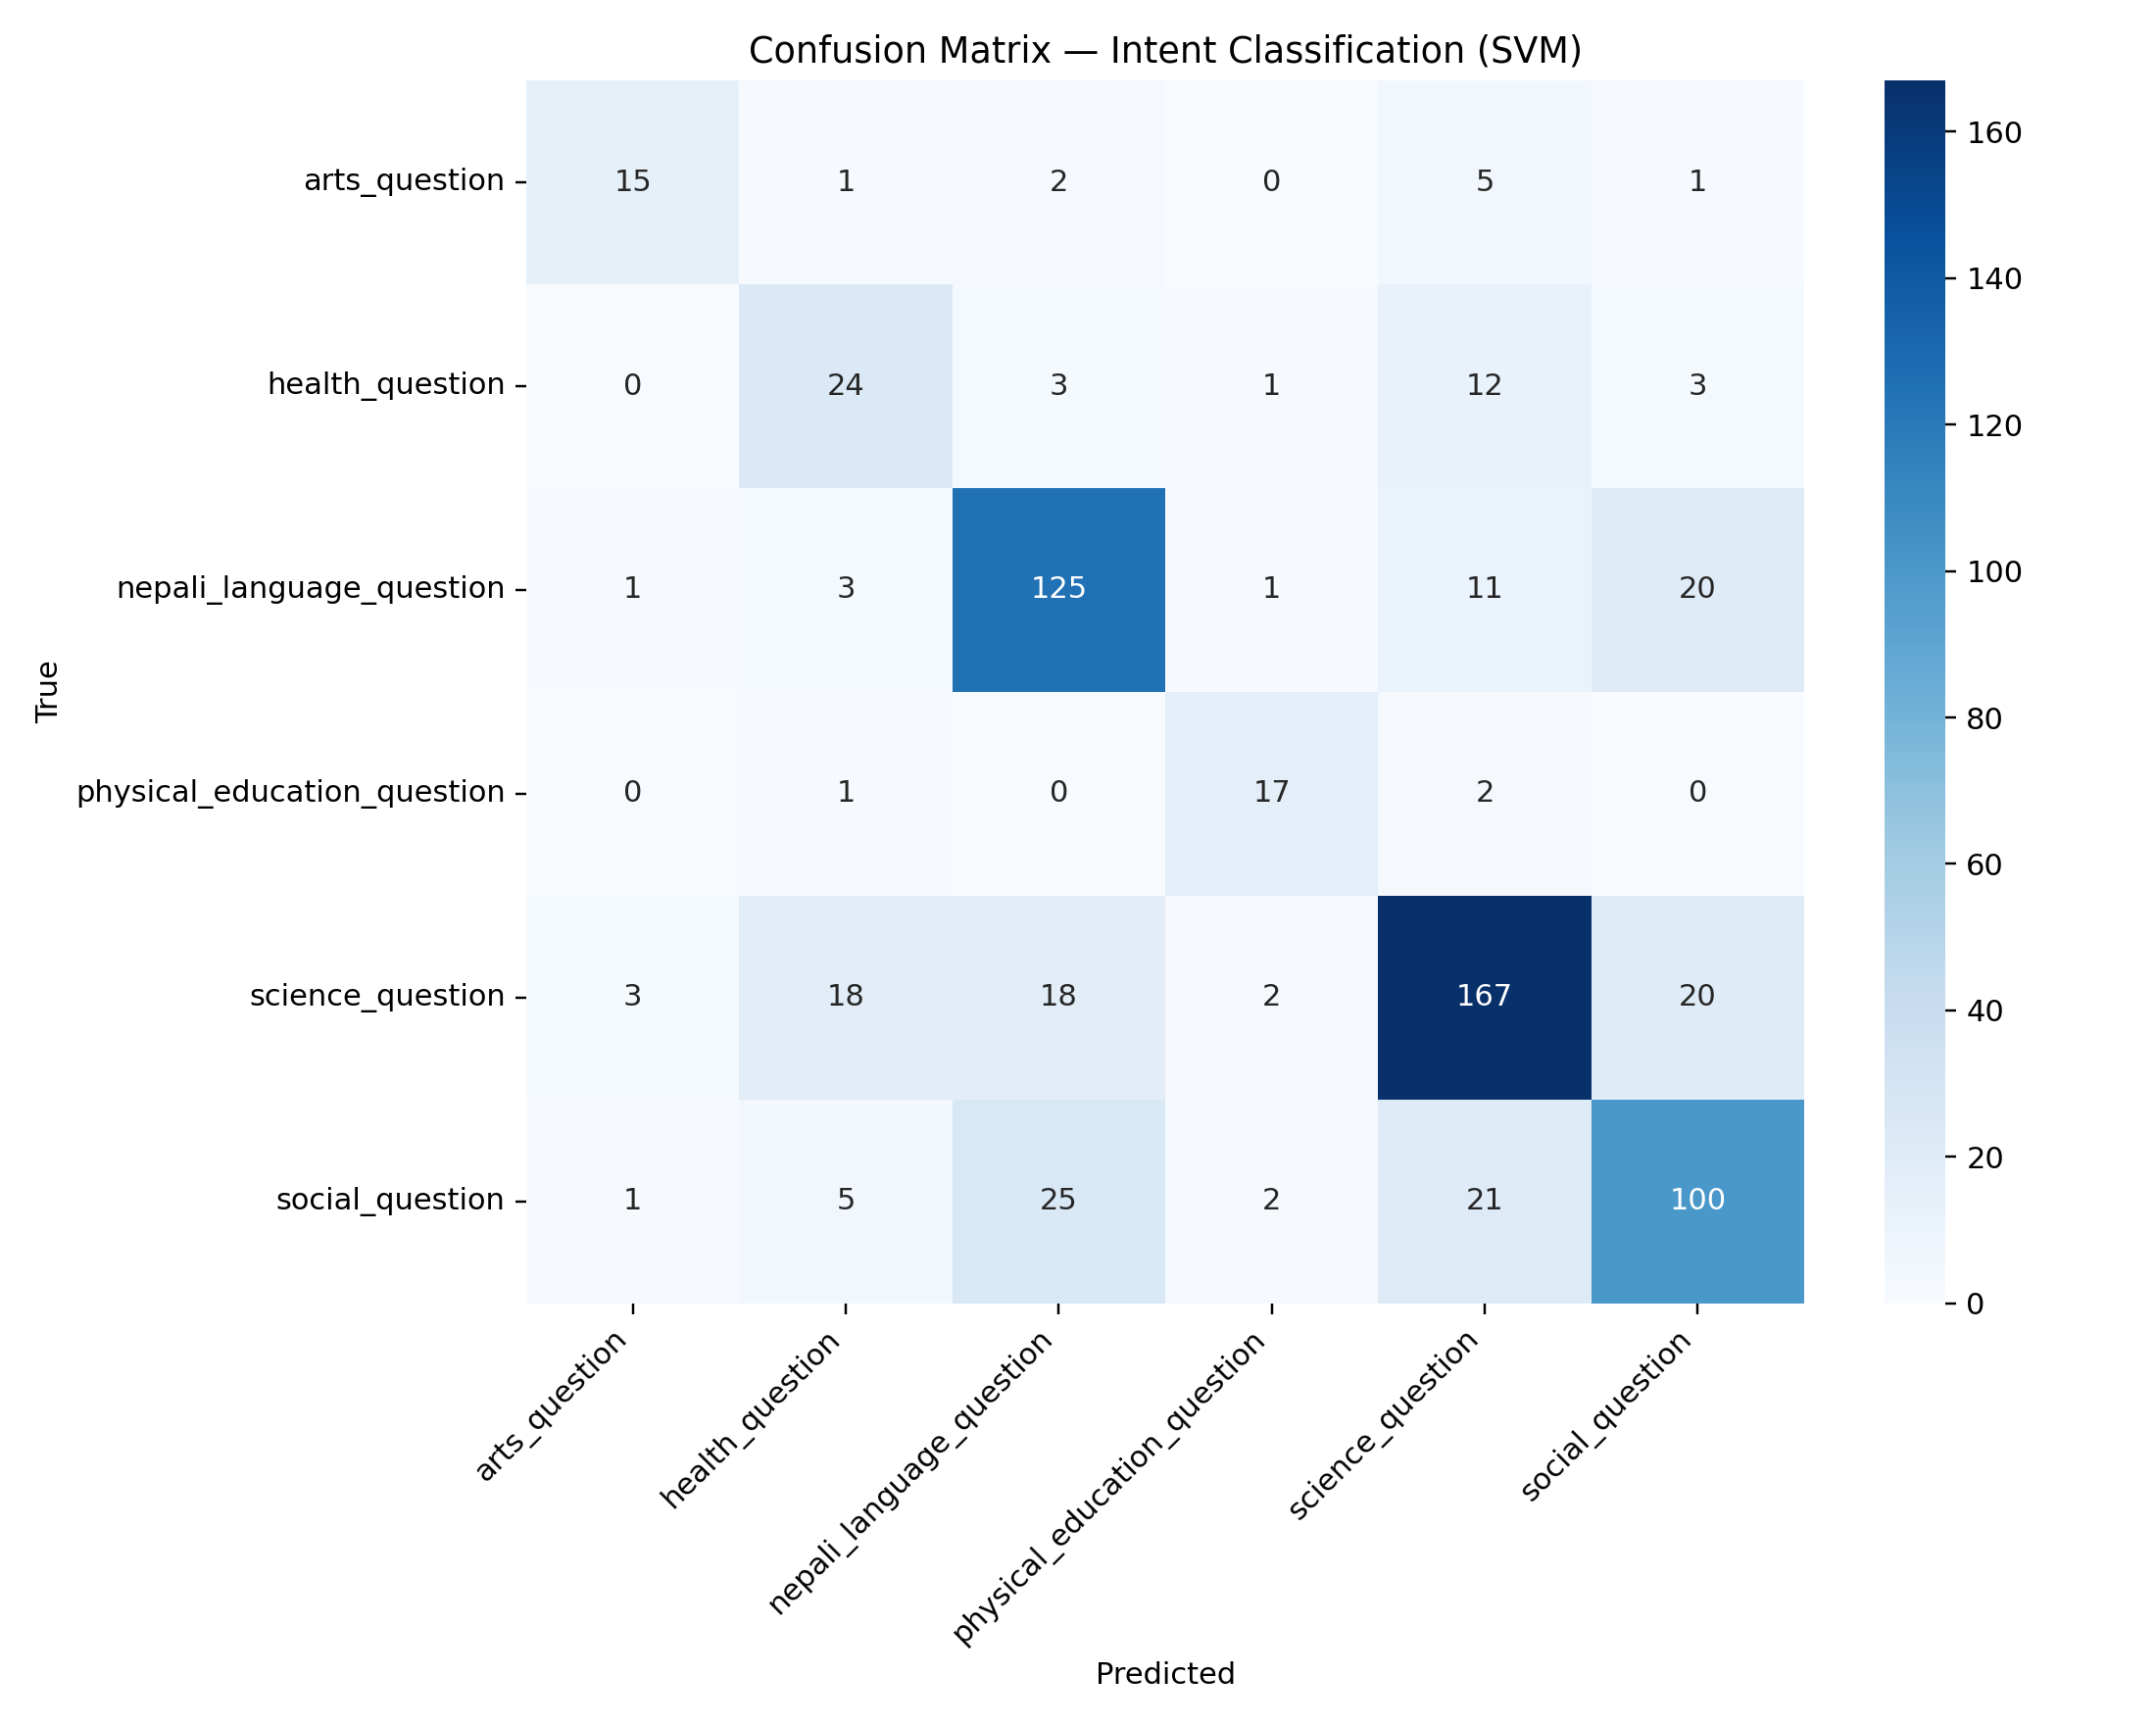
\includegraphics[width=\linewidth]{../outputs/confusion_matrix_eval.png}
\caption{Confusion matrix heatmap for the optimized SVM on the test split.}
\label{fig:cm}
\end{figure}

\subsection{Latency Benchmark (CPU, No TTS)}
Benchmarking over 50 queries (from \texttt{outputs/eval\_report.txt}) is summarized in Table~\ref{tab:latency}.

\begin{table}[ht]
\caption{Latency per Query (ms), CPU-only (No TTS)}
\label{tab:latency}
\centering
\begin{tabular}{lrr}
\toprule
Stage & Mean (ms) & P95 (ms) \\
\midrule
Intent classification & 20.0 & 26.1 \\
Retrieval & 1.8 & 2.6 \\
\textbf{Total} & \textbf{21.9} & \textbf{28.5} \\
\bottomrule
\end{tabular}
\end{table}

\section{Conclusion}
This work demonstrates that an offline Nepali student assistant can be implemented with classical machine learning methods while remaining fast and practical on CPU-only hardware. The optimized Linear SVM pipeline achieved 74.65\% test accuracy with 77.53\% macro F1 and maintained low per-query latency (21.9\,ms mean for intent + retrieval). The results support feasibility for low-resource immediate systems and establish a reproducible baseline for Nepali educational intent classification using SVM.

\section{Future Research}
Future improvements include: expanding the dataset (more grades, more intents, more diverse phrasing), formal ASR evaluation (e.g., WER on a Nepali speech test set) and robustness testing under classroom noise, further optimization of the SVM pipeline (feature experiments, calibration, and an ``unknown intent'' option), user studies with students/teachers, and improved retrieval with BM25 or hybrid offline methods where feasible.

\section*{Acknowledgment}
This project was completed as part of the STW7072CEM Machine Learning coursework at Softwarica College of IT \& E-Commerce (in collaboration with Coventry University).

\begin{thebibliography}{00}
\bibitem{smote} N.~V. Chawla, K.~W. Bowyer, L.~O. Hall, and W.~P. Kegelmeyer, ``SMOTE: Synthetic Minority Over-sampling Technique,'' \emph{Journal of Artificial Intelligence Research}, vol.~16, pp. 321--357, 2002.
\bibitem{joachims} T.~Joachims, ``Text Categorization with Support Vector Machines: Learning with Many Relevant Features,'' in \emph{Proc. ECML}, 1998, pp. 137--142.
\bibitem{sklearn} F.~Pedregosa \emph{et~al.}, ``Scikit-learn: Machine Learning in Python,'' \emph{JMLR}, vol.~12, pp. 2825--2830, 2011.
\bibitem{whisper} A.~Radford \emph{et~al.}, ``Robust Speech Recognition via Large-Scale Weak Supervision,'' in \emph{Proc. ICML}, 2023.
\bibitem{bm25} S.~Robertson, H.~Zaragoza, and M.~Taylor, ``Simple BM25 Extension to Multiple Weighted Fields,'' in \emph{Proc. CIKM}, 2004, pp. 42--49.
\end{thebibliography}

\appendices
\section{Reproducibility (Code Execution)}
The project contains scripts and artifacts to reproduce the results and figures.
\begin{verbatim}
python -m venv .venv
.\.venv\Scripts\Activate.ps1
pip install -r requirements.txt

# Data prep + EDA
python .\codes\data_prep.py

# Train optimized SVM
python .\codes\train_model.py

# Evaluate + generate figures + latency benchmark
python .\codes\evaluate_and_benchmark.py

# Launch GUI
python .\codes\app.py
\end{verbatim}

\end{document}

